% ============================================================================
% RA-6: Agent Simulation, Testing & Formal Verification
% arXiv Preprint — v0.9
% Date: 2026-04-19
% Revisions: addresses 22 annotations from Dr A. Sanyal (chair) review of v0.8
% ============================================================================
\documentclass[11pt,a4paper]{article}

% ---- Packages ----
\usepackage[utf8]{inputenc}
\usepackage[T1]{fontenc}
\usepackage{amsmath,amssymb,amsfonts,amsthm}
\usepackage{graphicx}
\usepackage{booktabs}
\usepackage{hyperref}
\usepackage{cleveref}
\usepackage{algorithm}
\usepackage{algorithmic}
\usepackage{listings}
\usepackage{xcolor}
\usepackage{tikz}
\usetikzlibrary{arrows.meta,positioning,shapes.geometric,fit,calc,
  automata}
\usepackage[margin=1in]{geometry}
\usepackage{natbib}
\bibliographystyle{plainnat}
\usepackage{tcolorbox}
\usepackage{enumitem}
\usepackage{mathtools}
\usepackage{multirow}

% ---- Theorem Environments ----
\newtheorem{definition}{Definition}[section]
\newtheorem{property}{Property}[section]

% ---- Custom Commands ----
\newcommand{\faos}{\textsc{FAOS}}
\newcommand{\asim}{\textsc{A-Sim}}
\newcommand{\agent}{\mathcal{A}}
\newcommand{\env}{\mathcal{E}}
\newcommand{\scenario}{\mathcal{S}}
\newcommand{\onto}{\mathcal{O}}
\newcommand{\verdict}{\mathcal{V}}
\newcommand{\cert}{\mathcal{C}}
\newcommand{\prop}{\varphi}
\newcommand{\inv}{\psi}

% ---- Metadata ----
\title{%
  Toward Pre-Deployment Assurance for Enterprise AI Agents:\\
  Ontology-Grounded Simulation and Trust Certification%
}

\author{
  Thanh Luong Tuan\thanks{Corresponding author. Email: tluongtuan@my.ggu.edu \quad ORCID: 0009-0000-1199-837X} \\
  \textit{Golden Gate University, San Francisco} \\
  \textit{Foundation AgenticOS (FAOS)}
  \and
  Abhijit Sanyal\thanks{Email: abhijit.sap@gmail.com \quad ORCID: 0009-0005-7520-5881} \\
  \textit{Associate Director, Data, Digital \& IT} \\
  \textit{Novartis Healthcare Pvt.\ Ltd., Hyderabad, India}
}

\date{April 2026}

% ============================================================================
\begin{document}
\maketitle

% ============================================================================
% ABSTRACT
% ============================================================================
\begin{abstract}
Pre-deployment verification of enterprise AI agents remains a critical
gap between large language model (LLM) capability benchmarking and
production deployment, where post-deployment monitoring,
human-in-the-loop controls, and prompt-level guardrails provide
limited assurance. We propose an ontology-grounded verification
framework combining three components: an Agent Operational Envelope
formalising the certification space across permissions, domain
constraints, safety properties, governance rules, and autonomy levels;
an ontology-to-scenario generation pipeline that derives regulatory,
operational, and adversarial test scenarios automatically; and a Trust
Certificate carrying a machine-verifiable attestation with graduated
deployment verdicts (Approved, Conditional, Rejected). A controlled
pilot across four regulated industries---Fintech, Banking, Insurance,
and Healthcare---instantiated as five industry-by-regulatory-regime
cells across the United States and Vietnam, generated 1{,}800
scenarios evaluated against 125 primary-source regulatory requirements
and 25 injected faults. Ontology-grounded generation (G4) achieved
48.3\% regulatory coverage versus 33.1\% for the persona-based
baseline ($p_c{=}.0006$) and the highest domain specificity
(4.77/5.0, $p{=}2{\times}10^{-6}$), while the coverage advantage over
baseline and retrieval-augmented prompting was not robust after
Bonferroni correction. Cross-validation across three LLM families
(Claude Sonnet~4, Qwen~2.5 72B, Gemma~4 26B; 5{,}400 total scenarios)
replicated the persona-versus-ontology pattern. The results establish
ontology-grounded scenario generation as a credible complement to
persona-based test suites for regulatory-intensive domains.
\end{abstract}

\noindent\textbf{Keywords:} AI Safety, Agent Verification, Formal
Methods, Ontology-Powered Testing, Simulation Engine, Agent Certification,
Enterprise AI, Runtime Verification

% ============================================================================
% 1. INTRODUCTION
% ============================================================================
\section{Introduction}
\label{sec:introduction}

Enterprise buyers considering autonomous AI agents face a paradox: the
more capable the agent, the greater the potential value and the
greater the risk. Insurance underwriting agents that approve policies,
financial advisors that execute trades, and healthcare triage agents
that prioritize patients all operate in domains where errors carry
regulatory, financial, and human consequences. The critical question
is not whether modern LLMs can perform such tasks but whether
operators can verify they will perform safely before granting
production access. We refer to this as the \emph{agent verification
problem}: providing pre-deployment assurance that an AI agent will
behave within acceptable bounds across the space of scenarios it may
encounter.

Existing approaches to enterprise agent safety remain inadequate for
this purpose. Post-deployment monitoring \citep{amodei2016concrete}
intervenes only after harm has occurred; human-in-the-loop gates
\citep{christiano2017deep} create bottlenecks and shift the
verification burden onto reviewers who may lack domain expertise; and
prompt-level guardrails \citep{bai2022constitutional} are
probabilistic rather than deterministic, and may be ignored under
adversarial or edge-case conditions. Safety-critical industries
solved an analogous problem decades ago through standards such as
DO-178C \citep{rierson2017developing}, IEC~62304 \citep{iec62304},
and ISO~26262 \citep{iso26262}, which mandate rigorous pre-deployment
verification. No analogous standard yet exists for enterprise AI
agents operating in regulated industries.

This paper proposes that industry ontologies---formal representations
of domain concepts, regulatory frameworks, and operational
constraints---provide the foundation for systematic agent
verification. Ontology-powered verification automatically derives
test scenarios from each industry's regulatory and operational
structure, producing industry-specific, evolvable test suites that
prompt-level guardrails cannot match. We pair this
generation approach with a machine-verifiable Trust Certificate that
attests to an agent's behavior within a formally defined operational
envelope, and present a controlled pilot study and three-model
cross-validation that empirically confirm the regulatory coverage and
industry specificity advantages of ontology-powered generation across
four regulated industries---Fintech, Banking, Insurance, and
Healthcare---and three LLM families.

% ============================================================================
% 2. RELATED WORK
% ============================================================================
\section{Related Work}
\label{sec:related-work}

\subsection{AI Safety and Alignment}

AI safety research has identified concrete problems in deploying
autonomous systems, including reward hacking, distributional shift,
and unsafe exploration \citep{amodei2016concrete}. Constitutional AI
\citep{bai2022constitutional} proposes training-time alignment through
principle-based self-critique, while RLHF \citep{christiano2017deep}
uses human preferences to shape model behavior. More recently,
\citet{weidinger2023sociotechnical} argue for sociotechnical
approaches to AI safety that consider the deployment context---not
just the model in isolation. Our work aligns with this perspective:
we verify agents (model + tools + context + domain ontology) within
their \emph{operational context}, not models in abstraction.

A critical gap in existing safety work is the transition from
\emph{model safety} to \emph{agent safety}. Models are evaluated on
benchmarks; agents are evaluated on deployment outcomes.
Recent benchmarks have begun to quantify this gap:
\citet{andriushchenko2025agentharm} demonstrate that leading LLMs are
``surprisingly compliant with malicious agent requests'' across 110
harmful tasks spanning 11 categories, while
\citet{zhang2025agentsafetybench} find that \emph{none} of 16 tested
LLM agents achieves a safety score above 60\% across 349 interaction
environments---identifying insufficient robustness and inadequate
risk awareness as core deficiencies.
\citet{chan2024visibility} identify ``visibility'' as a key challenge:
enterprise stakeholders cannot inspect what an LLM-based agent
``knows'' or predict how it will behave in novel scenarios. Our
Trust Certificate (\Cref{sec:safety-certificate}) directly
addresses this visibility gap by making verification results
inspectable, auditable, and enforceable.

\subsection{Formal Verification of AI Systems}

Formal verification of neural networks has advanced significantly,
with techniques for verifying robustness properties
\citep{huang2020survey, katz2017reluplex}, reachability analysis
\citep{tran2020nnv}, and abstract interpretation
\citep{singh2019abstract}. However, these techniques address
\emph{individual neural network properties} (e.g., robustness to
perturbation), not \emph{agent-level behavioral properties} (e.g.,
``the agent never approves a loan exceeding the applicant's
debt-to-income threshold'').

Model checking for multi-agent systems \citep{lomuscio2017mcmas}
provides temporal logic verification of agent protocols, but assumes
agents with well-defined transition functions---an assumption violated
by LLM-based agents whose behavior is stochastic and context-dependent.
\citet{dalrymple2024guaranteed} propose ``guaranteed safe AI'' through
world models and safety specifications, arguing that formal methods
must adapt to probabilistic systems rather than demand determinism.
Their framework of \emph{quantitative safety guarantees}---bounding
the probability of unsafe behavior rather than proving its
impossibility---directly informs our probabilistic bounded model
checking approach (\Cref{sec:formal-extensions}).

Our work bridges the gap between NN verification and agent
verification by defining \emph{behavioral envelopes} that constrain
the space of acceptable agent behaviors, then using simulation and
lightweight formal methods to verify adherence. The key insight is
that enterprise ontologies provide the \emph{specification language}
that NN verification lacks for agent-level properties.

\subsection{Agent Testing and Simulation}

Agent-based simulation has a rich history in computational social
science \citep{macal2010tutorial} and software testing
\citep{bertolino2007software}. Recent work on LLM agent evaluation
includes benchmark suites \citep{liu2023agentbench, shinn2023reflexion},
red-teaming methodologies \citep{perez2022red}, and simulation
environments for multi-agent interaction \citep{park2023generative}.

Recent work on \emph{agent sandboxing} addresses the safety dimension
directly. \citet{ruan2024identifying} propose ToolEmu, an LLM-emulated
sandbox that simulates tool execution to identify risks before
deployment---sharing our pre-deployment verification philosophy, though
without ontological grounding of the risk space. \citet{xi2023rise}
survey the rapidly expanding LLM-based agent literature, flagging
safety and trustworthiness as open challenges, while
\citet{wang2024survey} catalog evaluation methodologies across agent
capabilities and find that domain-specific evaluation remains
underdeveloped.
\citet{yuan2024rjudge} introduce R-Judge, a benchmark specifically
targeting safety risk awareness in LLM agents across 27 risk
scenarios. \citet{yin2025safeagentbench} extend safety evaluation
to embodied agents with SafeAgentBench (750 tasks, 10 hazard types),
finding that even the most safety-conscious baseline achieves only
10\% rejection of detailed hazardous tasks. These benchmarks share
our pre-deployment verification philosophy but lack two properties
our framework provides: (1)~\emph{domain-specific} regulatory
grounding (their risks are generic, not industry-specific), and
(2)~\emph{formal certification} (they produce scores, not auditable
safety attestations).

The most directly relevant commercial system is Lyzr's Agent
Simulation Engine (\asim{}), which executes 20,000+ simulations per
agent using compositional world models and multi-objective
reinforcement hardening \citep{lyzr2026}. \asim{} employs a
generic persona-by-scenario matrix approach: persona variations
(e.g., ``impatient customer,'' ``confused user'') are crossed with
scenario categories (e.g., ``refund request,'' ``complaint
escalation'') to generate test cases.

The present approach differs structurally: rather than generic
persona-scenario matrices, scenarios derive from \emph{formal industry
ontologies} that encode the actual regulatory frameworks, business
metrics, and domain-specific edge cases of each industry. The result
is a test suite that goes beyond behavioural surface coverage (``does
the agent respond politely?'') and into regulatory specifics (``does
the agent correctly apply BSA/AML thresholds when processing a
\$9,500 cash deposit?'').

Our ontology-to-scenario generation is an instance of
\emph{model-based testing} (MBT) \citep{utting2012taxonomy}, where
the model is an industry ontology rather than a state machine or UML
diagram. MBT's core advantage---systematic coverage derived from a
formal model---translates directly: the ontology serves as both the
specification (what to test) and the oracle (how to evaluate), a
dual role we explore further in \Cref{sec:discussion}.

\subsection{LLM-as-Judge Evaluation}

Our evaluation pipeline relies on LLM-as-judge
\citep{zheng2023judging}, in which a strong LLM evaluates the
outputs of another LLM against structured criteria. This approach
has become standard for scalable evaluation where human annotation
is cost-prohibitive. \citet{zheng2023judging} demonstrate that
strong LLMs (GPT-4-class) achieve $>80\%$ agreement with human
judges on open-ended quality assessment, though they identify
systematic biases including position bias, verbosity bias, and
self-enhancement bias.

For our domain---regulatory compliance assessment---the evaluation
task is more constrained than open-ended quality rating: the judge
receives an explicit regulation and determines whether a scenario
tests it (binary). This structured rubric design reduces the scope
for the biases identified by \citet{zheng2023judging}.
\citet{shankar2024validates} raise a deeper concern: who validates
the validators? They find that LLM-based evaluation criteria
frequently diverge from human preferences, especially on
domain-specific tasks.

A comprehensive survey by \citet{gu2024llmjudgesurvey} systematizes
approaches to improving LLM-as-Judge reliability, including consistency
enhancement, bias reduction, and domain-specific adaptation.
\citet{luo2025agentauditor} advance the state of the art with
AgentAuditor, a memory-augmented reasoning framework that achieves
\emph{human-level accuracy} on agent safety evaluation (NeurIPS~2025),
validated on their ASSEBench benchmark (2,293 annotated records,
15 risk types). More broadly, \citet{you2026agentjudge} survey the
emerging shift from LLM-as-a-Judge to \emph{Agent-as-a-Judge},
where evaluators employ planning, tool-augmented verification, and
multi-agent collaboration---capabilities that align with our
structured, ontology-grounded evaluation rubrics but that we
deliberately forgo in favor of reproducible, deterministic assessment.

We address the validator reliability concern partially through our
anti-circularity controls (E1) and acknowledge the need for human
expert calibration as future work (\Cref{sec:limitations}).

\subsection{Ontology Engineering and Knowledge Graphs}

Enterprise ontologies have evolved from formal knowledge
representation artifacts to operational components of AI systems.
Foundational work on graph-semantic web data models
\citep{sanyal2011graph} and on automating the conceptual-to-logical
translation of web data models \citep{sanyal2010automating}
established that domain ontologies can be derived systematically and
mapped to operational representations rather than authored ad~hoc.
\citet{hogan2021knowledge} provide a comprehensive survey of
knowledge graphs---the runtime instantiation of ontologies---covering
construction, storage, querying, and application, establishing the
infrastructure that our industry ontologies build upon.
\citet{pan2024unifying} survey the convergence of LLMs and knowledge
graphs, identifying two directions: KG-enhanced LLMs (using
structured knowledge to improve LLM outputs) and LLM-enhanced KGs
(using LLMs to construct or complete knowledge graphs). Our work
contributes a third direction: \emph{ontology-powered LLM
verification}---using structured knowledge not to improve the
agent's outputs, but to \emph{verify} them. This verification
perspective is largely absent from the LLM-KG unification literature.

\subsection{AI Governance Frameworks}

Regulatory frameworks for AI systems are rapidly maturing.
The NIST AI Risk Management Framework \citep{nist2023ai} sets out a
voluntary framework organized around four functions---Govern, Map,
Measure, Manage---that aligns closely with our verification approach:
ontology-to-scenario generation implements the ``Map'' and ``Measure''
functions, while the Trust Certificate provides the ``Manage''
artifact. The EU AI Act \citep{euaiact2024} classifies AI systems by
risk level and mandates conformity assessments for high-risk systems;
our graduated certification framework (Approved/Conditional/Rejected)
is designed to satisfy Article~9 (Risk Management) and Article~15
(Accuracy, Robustness, Cybersecurity) requirements. Singapore's
Model AI Governance Framework \citep{imda2020model} emphasizes
human oversight proportional to risk---a principle reflected in our
autonomy level semantics (\Cref{tab:autonomy-levels}).
ISO/IEC~42001:2023 \citep{iso42001} specifies AI management system
requirements, including risk assessment processes that our simulation
gate can operationalize.

Agent-governance activity accelerated sharply in 2025--2026.
\citet{owasp2025agentic} published the first formal risk taxonomy
for autonomous AI agents, identifying 10 critical risks including
goal hijacking, tool misuse, identity abuse, memory poisoning, and
rogue agents (threat model T01--T17, 100+ expert contributors).
NIST launched the AI Agent Standards Initiative in February 2026
\citep{nist2026agents}, focusing on identity, security, and
interoperability standards for autonomous agents.
\citet{microsoft2026agt} released the Agent Governance Toolkit,
the first open-source system addressing all 10 OWASP agentic risks
with deterministic, sub-millisecond policy enforcement---including
execution sandboxing, compliance grading, and agent-to-agent
communication security.

At the national level, Vietnam passed Law~No.~134/2025/QH15 on
Artificial Intelligence \citep{vnailaw2025}---one of the first
standalone AI laws in Southeast Asia, effective March~1, 2026. The
law sets a three-tier risk classification (low/medium/high) and
mandates conformity assessments, human oversight, and registration
in a National AI Database for high-risk systems.
Financial services AI (including banking and insurance) is
classified as high-risk with an 18-month grace period (full
compliance by September~2027). Decree~94/2025/N\DJ-CP
\citep{vnfintechsandbox2025} further creates a regulatory sandbox
for AI-enabled banking services. These Vietnamese
regulations directly motivate our inclusion of banking~(VN) and
insurance~(VN) as experimental verticals: they represent a
regulatory regime where pre-deployment AI verification is not
optional but legally mandated.

These frameworks share a common gap: they specify \emph{what} to
verify but not \emph{how}. OWASP identifies risks; NIST calls for
standards; Microsoft provides runtime enforcement; Vietnam's AI Law
mandates conformity assessments. None addresses \emph{pre-deployment
verification} through systematic test generation from domain
ontologies. Our ontology-powered approach provides a concrete ``how''
that maps framework requirements to executable verification
scenarios, complementing these governance mechanisms with
design-time assurance.

\subsection{Safety Standards for Critical Systems}

Safety-critical software industries have developed rigorous
verification standards:

\begin{itemize}
  \item \textbf{DO-178C} (avionics): Defines 5 software levels
    (A--E) with increasing verification rigor; Level A requires
    modified condition/decision coverage (MC/DC) testing
    \citep{rierson2017developing}.

  \item \textbf{IEC 62304} (medical devices): Classifies software
    into safety classes (A, B, C) with corresponding verification
    requirements \citep{iec62304}.

  \item \textbf{ISO 26262} (automotive): Defines Automotive Safety
    Integrity Levels (ASIL A--D) with verification methods including
    fault injection and formal verification \citep{iso26262}.
\end{itemize}

No analogous standard exists for enterprise AI agents. We argue that
the emerging EU AI Act \citep{euaiact2024}, which classifies AI
systems by risk level, provides a regulatory impetus for developing
such standards. Our Trust Certificate framework is designed to
be compatible with EU AI Act high-risk requirements.

% ============================================================================
% 3. GAPS IN EXISTING APPROACHES
% ============================================================================
\section{Gaps in Existing Approaches}
\label{sec:gaps}

The literature surveyed in \Cref{sec:related-work} reveals six major
gaps addressed in this study. \emph{First}, existing approaches do
not comprehensively formalize the operational envelope within which an
AI agent is authorized and validated to operate, leaving safety claims
insufficiently scoped and difficult to enforce. \emph{Second}, current
agent-safety benchmarks \citep{liu2023agentbench, yuan2024rjudge,
andriushchenko2025agentharm, zhang2025agentsafetybench,
yin2025safeagentbench} rely heavily on manually curated test cases,
limiting scalability across the large number of industry verticals
required for enterprise deployment and resulting in fragmented rather
than systematic regulatory coverage. \emph{Third}, existing evaluation
frameworks rarely provide machine-verifiable and cryptographically
bound attestations linking a specific agent version to validated
behavioural properties under defined operational constraints.
\emph{Fourth}, many current platforms implement safety controls
primarily at the application layer, which may be circumvented under
orchestration or configuration failures, while lacking
infrastructure-level deployment gates for uncertified agents.
\emph{Fifth}, simulation-based approaches provide statistical evidence
rather than formal guarantees, whereas most neural-network
verification methods \citep{huang2020survey, katz2017reluplex,
tran2020nnv, singh2019abstract} focus on bounded model-level
properties rather than behavioural invariants across multi-step agent
workflows. \emph{Sixth}, most empirical studies on agent safety
evaluate a single LLM family, leaving unresolved whether observed
outcomes arise from model-specific latent knowledge or from structural
properties of the verification methodology itself. Collectively, the
proposed framework components described in
\Crefrange{sec:proposed-framework}{sec:simulation-architecture}
address Gaps~(1)--(4), while the evaluation methodology in
\Cref{sec:eval-framework} addresses Gaps~(5)--(6).

% ============================================================================
% 4. PROPOSED FRAMEWORK
% ============================================================================
\section{Proposed Enterprise Agentic AI Framework}
\label{sec:proposed-framework}

\subsection{Framework Overview}

Three components make up the proposed framework for pre-deployment
verification of enterprise AI agents: the \emph{Agent Operational
Envelope} (\Cref{sec:operational-envelope}) formalizes the space
within which an agent is certified to operate;
\emph{Ontology-to-Scenario Generation}
(\Cref{sec:scenario-generation}) automatically derives test scenarios
from industry ontologies; and the \emph{Trust Certificate}
(\Cref{sec:safety-certificate}) provides a machine-verifiable
attestation that binds an agent version to its verification evidence.
\Cref{sec:simulation-architecture} then describes the implementation
architecture that executes this framework, and
\Cref{sec:eval-framework} the quantitative and empirical evaluation
frameworks that establish trust in the result.

\subsection{Agent Operational Envelope}
\label{sec:operational-envelope}

We introduce the concept of an \emph{operational envelope}: the
formally defined space within which an agent is certified to operate.

\subsubsection{Formal Definition}

\begin{definition}[Agent Operational Envelope]
  An agent operational envelope $\env_\agent$ for agent $\agent$
  operating under ontology $\onto$ is defined as a tuple:
  \begin{equation}
    \env_\agent = \langle \Pi, \Sigma, \Phi, \Gamma, \Lambda \rangle
  \end{equation}
  where:
  \begin{itemize}
    \item $\Pi$: \textbf{Permission boundary} --- the set of actions
      the agent is authorized to perform
    \item $\Sigma$: \textbf{Domain scope} --- the ontological domains
      within which the agent may reason
    \item $\Phi$: \textbf{Safety properties} --- invariants that must
      hold across all agent executions
    \item $\Gamma$: \textbf{Governance constraints} --- regulatory
      rules that bound agent decisions
    \item $\Lambda$: \textbf{Autonomy level} --- the degree of
      independent action permitted ($L0$--$L3$)
  \end{itemize}
\end{definition}

\subsubsection{Deriving Envelopes from Ontologies}

Each component of $\env_\agent$ is derived from the enterprise
ontology $\onto = \langle \mathcal{R}, \mathcal{D}, \mathcal{I} \rangle$
(as defined in our companion paper on neurosymbolic architectures).
We illustrate with a concrete fintech example---a BSA/AML Compliance
Analyst agent:

\begin{align}
  \Pi &= \text{actions}(\mathcal{R}_{r_i}.\alpha_i)
    & \text{(from role approval authority)} \\
  \Sigma &= \text{domains}(\mathcal{D}.\mathcal{V})
    & \text{(from domain verticals)} \\
  \Phi &= \text{invariants}(\mathcal{D}.G)
    & \text{(from governance constraints)} \\
  \Gamma &= \text{regulations}(\mathcal{D}.G)
    & \text{(from regulatory frameworks)} \\
  \Lambda &= \text{level}(\agent.\text{config})
    & \text{(from agent configuration)}
\end{align}

\begin{tcolorbox}[title=Example: Fintech Compliance Analyst Envelope,
  colback=blue!5, colframe=blue!40]
\small
\begin{align*}
  \Pi &= \{\text{flag\_suspicious}, \text{file\_CTR}, \text{file\_SAR},
    \text{escalate}\} \\
    &\quad \text{(NOT: approve\_loan, execute\_trade)} \\
  \Sigma &= \{\text{BSA/AML}, \text{KYC}, \text{sanctions}\} \\
  \Phi &= \{\text{``never disclose SAR filing to subject''},\\
    &\quad\phantom{\{} \text{``always verify identity before account access''}\} \\
  \Gamma &= \{31\text{ CFR }\S1010\text{--}1020, \text{ OCC 2013-29},
    \text{ FinCEN guidance}\} \\
  \Lambda &= L2 \text{ (Execute: autonomous within bounds, escalate
    when uncertain)}
\end{align*}
\end{tcolorbox}

\noindent This envelope is \emph{automatically derivable} from the
fintech ontology---the same ontology used to generate test scenarios
in our pilot study (\Cref{sec:empirical}). The permission boundary $\Pi$
comes from the role's \texttt{approval\_authority} field; the
governance constraints $\Gamma$ from the ontology's regulatory layer.

\subsubsection{Autonomy Level Semantics}

The autonomy level $\Lambda$ determines the agent's decision authority
within its permission boundary:

\begin{table}[htbp]
\centering
\caption{Autonomy Level Semantics}
\label{tab:autonomy-levels}
\begin{tabular}{@{}clp{6cm}@{}}
\toprule
\textbf{Level} & \textbf{Name} & \textbf{Operational Semantics} \\
\midrule
$L0$ & Suggest & Agent produces recommendations; all actions require
  human approval before execution \\
$L1$ & Plan & Agent decomposes tasks and proposes execution plans;
  human approves plan execution \\
$L2$ & Execute & Agent executes within defined boundaries; escalates
  when confidence falls below threshold \\
$L3$ & Delegate & Agent operates fully autonomously within envelope;
  reports outcomes post-execution \\
\bottomrule
\end{tabular}
\end{table}

\begin{property}[Autonomy Monotonicity --- Design Requirement]
\label{prop:autonomy-monotonicity}
  We impose as a design requirement that the verification configuration for an agent at level $\Lambda_j$ be strictly more demanding than at level $\Lambda_i$ when $j > i$:
  \begin{equation}
    \Lambda_j > \Lambda_i \implies |\scenario(\Lambda_j)| >
      |\scenario(\Lambda_i)| \wedge \theta_{\text{pass}}(\Lambda_j) >
      \theta_{\text{pass}}(\Lambda_i).
  \end{equation}
  This is a framework-level axiom (the scenario budget and pass threshold are engineering inputs set per autonomy tier), not a theorem derived from the Operational Envelope definition.
\end{property}

\subsubsection{Operational Envelope as Trust Attestation}

The operational envelope functions as a \emph{trust attestation} between
the agent and the enterprise: a precise statement of what the agent
is permitted to do, where it may reason, what invariants it must
preserve, and which regulatory rules bound its decisions. An execution
trace conforms to this attestation if and only if every step lies
within the envelope:

\begin{definition}[Envelope Compliance]
  An agent execution trace $\tau = \langle s_0, a_0, s_1, a_1,
  \ldots, s_n \rangle$ is \emph{envelope-compliant} if and only if:
  \begin{equation}
    \forall i \in [0, n]: a_i \in \Pi \wedge
      \text{domain}(s_i) \subseteq \Sigma \wedge
      \bigwedge_{\prop \in \Phi} \prop(s_i) \wedge
      \bigwedge_{\gamma \in \Gamma} \gamma(s_i, a_i)
  \end{equation}
\end{definition}

% ============================================================================
% 4.2 ONTOLOGY-TO-SCENARIO GENERATION (was Section 4)
% ============================================================================
\subsection{Ontology-to-Scenario Generation}
\label{sec:scenario-generation}

A key innovation of our framework is the automatic generation of test
scenarios from industry ontologies, eliminating the manual test
authoring bottleneck.

\subsubsection{Scenario Taxonomy}

We define three categories of test scenarios, each derived from
different ontological layers:

\begin{enumerate}
  \item \textbf{Regulatory scenarios} ($\scenario_R$): Derived from
    the governance constraints in the Domain Ontology ($\mathcal{D}.G$).
    Test whether the agent correctly applies regulatory requirements.
    \begin{itemize}
      \item Banking: BSA/AML transaction thresholds, KYC identity
        verification, CFPB fair lending, OFAC sanctions screening
      \item Healthcare: HIPAA privacy rules, EMTALA emergency
        treatment, Stark Law referral restrictions
      \item Insurance: NAIC solvency requirements, state DOI rate
        filing, claims adjudication guidelines
    \end{itemize}

  \item \textbf{KPI/Operational scenarios} ($\scenario_K$): Derived
    from the metrics definitions in the Domain Ontology ($\mathcal{D}.M$).
    Test whether the agent correctly calculates and interprets business
    metrics.
    \begin{itemize}
      \item ``Calculate the combined ratio given these loss and expense
        figures'' (insurance)
      \item ``Assess whether this NRR trend indicates churn risk''
        (SaaS)
      \item ``Evaluate OEE given these downtime and defect rates''
        (manufacturing)
    \end{itemize}

  \item \textbf{Adversarial scenarios} ($\scenario_A$): Generated
    to test agent resilience against boundary conditions and attacks.
    \begin{itemize}
      \item Prompt injection: attempts to override agent instructions
      \item Data exfiltration: requests for unauthorized data access
      \item Regulatory bypass: social engineering to skip compliance
        checks
      \item Role confusion: attempting to invoke actions outside the
        agent's approval authority
    \end{itemize}
\end{enumerate}

\subsubsection{Generation Algorithm}

\begin{algorithm}
\caption{Ontology-to-Scenario Generation}
\label{alg:scenario-gen}
\begin{algorithmic}[1]
\REQUIRE Industry ontology $\onto$, agent envelope $\env_\agent$
\ENSURE Scenario set $\scenario$
\STATE $\scenario \gets \emptyset$
\FORALL{regulation $\gamma \in \onto.\mathcal{D}.G$}
  \STATE $\scenario_R \gets \textsc{GenRegulatoryScenarios}(
    \gamma, \env_\agent.\Pi)$
  \COMMENT{Generate positive and negative test cases per regulation}
  \STATE $\scenario \gets \scenario \cup \scenario_R$
\ENDFOR
\FORALL{metric $m \in \onto.\mathcal{D}.M$}
  \STATE $\scenario_K \gets \textsc{GenKPIScenarios}(
    m, m.\text{healthy\_range}, m.\text{world\_class})$
  \COMMENT{Test metric calculation and interpretation}
  \STATE $\scenario \gets \scenario \cup \scenario_K$
\ENDFOR
\FORALL{action $a \in \env_\agent.\Pi$}
  \STATE $\scenario_A \gets \textsc{GenAdversarialScenarios}(a)$
  \COMMENT{Boundary conditions, injection, bypass attempts}
  \STATE $\scenario \gets \scenario \cup \scenario_A$
\ENDFOR
\STATE $\scenario \gets \textsc{Deduplicate}(\scenario)$
\RETURN $\scenario$
\end{algorithmic}
\end{algorithm}

Each regulatory constraint $\gamma$ generates at minimum two scenarios:
a \emph{positive case} (the agent should apply the regulation correctly)
and a \emph{negative case} (the agent should detect and reject a
regulatory violation). For regulations with numeric thresholds (e.g.,
BSA/AML \$10,000 reporting threshold), additional \emph{boundary cases}
are generated at $\text{threshold} \pm \epsilon$.

\paragraph{Information hierarchy.}
\Cref{alg:scenario-gen} represents the richest information condition
for scenario generation (G4 in our empirical evaluation,
\Cref{sec:empirical}). We can formalize the information available to
alternative generation strategies as a strict hierarchy:

\begin{equation}
  \text{I}_{\text{G1}} \subset \text{I}_{\text{G2}} \subset
  \text{I}_{\text{G3}} \subset \text{I}_{\text{G4}}
\end{equation}

\noindent where:
\begin{itemize}
  \item $\text{I}_{\text{G1}} = \{r, d\}$: agent role $r$ and
    industry domain name $d$ only (baseline LLM knowledge)
  \item $\text{I}_{\text{G2}} = \text{I}_{\text{G1}} \cup \{P, C\}$:
    adds persona set $P$ and scenario category set $C$
    (behavioral coverage matrix)
  \item $\text{I}_{\text{G3}} = \text{I}_{\text{G1}} \cup
    \{\text{chunks}(\onto)\}$: adds unstructured text extracted from
    the ontology (simulating RAG retrieval)
  \item $\text{I}_{\text{G4}} = \text{I}_{\text{G1}} \cup
    \{\onto' \subseteq \onto\}$: adds the full structured ontology
    (with holdout partition $\onto' = (1 - h) \cdot \onto$ for
    anti-circularity, where $h = 0.30$)
\end{itemize}

\noindent The key distinction is \emph{structural}: G3 receives the
same ontological \emph{content} as G4, but in flattened text form.
G4 receives the three-layer structure ($\langle \mathcal{R},
\mathcal{D}, \mathcal{I} \rangle$), enabling \Cref{alg:scenario-gen}'s
systematic traversal of regulatory constraints, metrics, and
permission boundaries. The hypothesis that structure matters above
and beyond content is empirically testable and is a primary question
of our pilot study.

\subsubsection{Coverage Analysis}

Ontology-driven generation enables formal coverage analysis:

\begin{definition}[Regulatory Coverage]
  The regulatory coverage of a scenario set $\scenario$ against
  ontology $\onto$ is:
  \begin{equation}
    \text{RC}(\scenario, \onto) = \frac{|\{\gamma \in \onto.\mathcal{D}.G
      \mid \exists s \in \scenario: s \text{ tests } \gamma\}|}{
      |\onto.\mathcal{D}.G|}
  \end{equation}
\end{definition}

Based on structural analysis of the \faos{} ontologies, the proposed
algorithm is estimated to generate 100+ scenarios per industry
vertical, with the potential for high regulatory coverage across
banking (Federal Reserve, OCC, FDIC, CFPB, FinCEN, SEC, FINRA,
Basel), insurance (NAIC, state DOI, RBC, ORSA, SAP, market conduct),
and healthcare (HIPAA, EMTALA, Stark Law, HITECH). We validate
these coverage estimates empirically in \Cref{sec:empirical},
comparing ontology-powered generation (G4) against three alternative
strategies across a ground-truth checklist of 125 regulatory
requirements (25 per industry) curated from primary sources.

% ============================================================================
% 4.3 TRUST CERTIFICATE
% ============================================================================
\subsection{Trust Certificate}
\label{sec:safety-certificate}

We formalize the concept of a Trust Certificate---a machine-verifiable
attestation of agent safety binding a specific agent version to its
verification evidence.

\subsubsection{Certificate Structure}

\begin{definition}[Trust Certificate]
  A Trust Certificate $\cert$ for agent $\agent$ is a tuple:
  \begin{equation}
    \cert_\agent = \langle \env_\agent, \scenario, \mathbf{R},
      \verdict, t, \text{sig} \rangle
  \end{equation}
  where:
  \begin{itemize}
    \item $\env_\agent$: The operational envelope under which
      certification was performed
    \item $\scenario$: The scenario set executed during verification
    \item $\mathbf{R}$: The results matrix (per-scenario pass/fail
      with judge evaluations)
    \item $\verdict$: The certification verdict
    \item $t$: The certification timestamp
    \item $\text{sig}$: A cryptographic signature binding the
      certificate to the specific agent version
  \end{itemize}
\end{definition}

\subsubsection{Verdict Framework}

The certification verdict $\verdict$ is determined by aggregate
simulation results:

\begin{equation}
  \verdict(\mathbf{R}) = \begin{cases}
    \textsc{Approved} & \text{if } \text{pass\_rate}(\mathbf{R})
      \geq \theta_{\text{high}} \\
    \textsc{Conditional} & \text{if } \theta_{\text{low}} \leq
      \text{pass\_rate}(\mathbf{R}) < \theta_{\text{high}} \\
    \textsc{Rejected} & \text{if } \text{pass\_rate}(\mathbf{R})
      < \theta_{\text{low}}
  \end{cases}
\end{equation}

In the \faos{} implementation, $\theta_{\text{high}} = 0.95$ and
$\theta_{\text{low}} = 0.80$. The intermediate verdict
\textsc{Conditional} requires manual review by an L3-authorized
human operator before production deployment.

\subsubsection{Verdict Enforcement: The Simulation Gate}

The simulation gate is an \emph{architectural enforcement point}
that blocks agent deployment based on certification verdict:

\begin{equation}
  \text{deploy}(\agent) = \begin{cases}
    \text{allow} & \text{if } \verdict = \textsc{Approved} \\
    \text{require\_L3\_approval} & \text{if } \verdict =
      \textsc{Conditional} \\
    \text{block} & \text{if } \verdict = \textsc{Rejected}
  \end{cases}
\end{equation}

This gate is designed to operate at the infrastructure level
(enforced in the Rust-native AgentOS runtime) rather than the
application level, so it cannot be bypassed by application-layer
code.
The gate would be environment-aware: enforced in \texttt{production}
and \texttt{customer-vpc} environments, skipped in \texttt{staging}
and \texttt{development}.

\subsubsection{Certificate Properties}

A well-formed Trust Certificate satisfies four properties.
\emph{Completeness:} the scenario set $\scenario$ achieves regulatory
coverage $\text{RC}(\scenario, \onto) \geq 0.95$ for all applicable
regulatory frameworks. \emph{Freshness:} the certificate timestamp
$t$ lies within the validity window
$t_{\text{current}} - t \leq \Delta t_{\text{max}}$, so certificate
expiry forces re-verification whenever ontologies or agent code
change. \emph{Version Binding:} the cryptographic signature
$\text{sig}$ binds the certificate to a specific agent version
(code hash + model version + ontology version), invalidating the
certificate on any change. \emph{Non-Transferability:} a certificate
$\cert_{\agent_i}$ is valid only for agent $\agent_i$ and cannot be
applied to $\agent_j \neq \agent_i$.

\emph{The following four statements are framework design requirements that a valid Trust Certificate must satisfy; they are not theorems derived from the definition above, and the pilot study does not empirically validate them ($\theta_{\text{Completeness}}{=}0.95$ is proposed, not achieved by any agent in the pilot).}

\begin{property}[Completeness --- Design Requirement]
  $\text{RC}(\scenario, \onto) \geq 0.95$ for all applicable regulatory frameworks.
\end{property}

\begin{property}[Freshness --- Design Requirement]
  $t_{\text{current}} - t \leq \Delta t_{\text{max}}$.
\end{property}

\begin{property}[Version Binding --- Design Requirement]
  $\text{sig}$ binds $\cert$ to a specific $(\text{code hash}, \text{model version}, \text{ontology version})$ triple; any change invalidates $\cert$.
\end{property}

\begin{property}[Non-Transferability --- Design Requirement]
  $\cert_{\agent_i}$ is valid only for $\agent_i$; $\agent_j \neq \agent_i \implies \cert_{\agent_i}\ \text{inapplicable}$.
\end{property}

% ============================================================================
% 5. PROPOSED IMPLEMENTATION ARCHITECTURE (was Section 6)
% ============================================================================
\section{Proposed Implementation Architecture}
\label{sec:simulation-architecture}

This section presents the implementation architecture for executing
the framework of \Cref{sec:proposed-framework}. The architecture
addresses gap~(4) of \Cref{sec:gaps}: an infrastructure-level
deployment gate that cannot be bypassed by application code.

\subsection{System Overview}

We propose a bilingual simulation architecture for the \faos{}
platform: a Rust-native simulation runner (for execution performance
and sandboxing) paired with a Python LLM-as-judge evaluator (for
semantic assessment), orchestrated via Temporal workflows for
durability. The LLM-as-judge component has been empirically validated
in our RA-3 pilot study \citep{luong2026neurosymbolic}; the
simulation runner and deployment gate are proposed designs.

\subsection{Simulation Runner}

The proposed Rust-native runner provides four execution guarantees.
\emph{Concurrency control:} bounded parallelism via
\texttt{tokio::Semaphore(10)} limits concurrent sandbox executions and
prevents resource exhaustion. \emph{Sandbox isolation:} each scenario
executes in an isolated sandbox environment with controlled tool
access. \emph{Timeout enforcement:} per-scenario timeout (default
60\,s, configurable per industry) with deterministic cleanup ensures
no scenario stalls the suite. \emph{Crash recovery:} Temporal workflow
durability ensures simulation state survives runner crashes and
resumes from the last checkpoint.

\subsection{LLM-as-Judge Evaluator}

Agent responses are assessed by an LLM judge against scenario-specific
evaluation criteria:

\begin{equation}
  \text{judge}(a, s) = \langle \text{pass} \in \{0, 1\},
    \text{score} \in [0, 1], \text{rationale} \in \text{String} \rangle
\end{equation}

The judge evaluates each response along four dimensions, each phrased
as a verifiable assertion. \emph{Regulatory compliance:} the response
correctly applies all applicable regulations to the scenario.
\emph{Domain accuracy:} domain terms and metrics are used correctly
according to the industry ontology. \emph{Safety boundary:} the
response remains within the agent's operational envelope.
\emph{Adversarial resilience:} the agent resists manipulation attempts
and refuses unauthorized actions.

In our pilot study (\Cref{sec:empirical}), we implement five
specialized judge variants that decompose this general
evaluator into measurable dimensions:

\begin{table}[htbp]
\centering
\caption{LLM-as-Judge variants used in the pilot study.}
\label{tab:judge-variants}
\begin{tabular}{@{}llll@{}}
\toprule
\textbf{Judge} & \textbf{Input} & \textbf{Output} & \textbf{DV} \\
\midrule
RC judge & regulation $+$ scenario & binary $+$ rationale & RC \\
ISS judge & scenario $+$ industry & 1--5 score & ISS \\
AC judge & scenario & category or null & AC \\
FDR-design & fault spec $+$ scenario & binary & FDR-d \\
FDR-exec & fault $+$ agent response & binary & FDR-e \\
\bottomrule
\end{tabular}
\end{table}

\noindent All judge variants use temperature $T=0.0$ for
deterministic evaluation. Each receives a structured rubric
constraining its assessment scope, following the recommendations
of \citet{zheng2023judging} for reducing LLM-as-judge bias.

\subsection{Coverage Reporting}

The proposed coverage reporter produces per-vertical analysis:

\begin{equation}
  \text{coverage}(\agent, \onto) = \langle
    \text{RC}_{\text{reg}},
    \text{RC}_{\text{kpi}},
    \text{RC}_{\text{adv}},
    \text{RC}_{\text{total}} \rangle
\end{equation}

\noindent where each component measures the percentage of ontological
elements covered by passing test scenarios. This report is included
in the Trust Certificate.

\subsection{Observability}

The simulation engine exports four Prometheus metrics for operational
monitoring: \texttt{simulation\_scenarios\_total} (counter of all
scenarios executed, labeled by verdict and industry),
\texttt{simulation\_scenarios\_failed} (counter of failed scenarios,
labeled by failure category), \texttt{simulation\_sandbox\_crashes}
(counter of sandbox crashes, indicating infrastructure rather than
agent issues), and \texttt{simulation\_duration\_seconds} (histogram
of per-scenario execution time).

% ============================================================================
% 6. PROPOSED EVALUATION FRAMEWORK FOR TRUST CREATION
% (was Section 7 Toward Formal Verification + Section 8 Empirical Evaluation)
% ============================================================================
\section{Proposed Evaluation Framework for Trust Creation}
\label{sec:eval-framework}

The framework of \Cref{sec:proposed-framework} specifies what to
verify; the architecture of \Cref{sec:simulation-architecture}
specifies how to execute the verification. This section presents the
two complementary evaluation frameworks that together establish trust
in the resulting Trust Certificate. The Quantitative Evaluation
Framework (\Cref{sec:formal-extensions}) provides mathematical
guarantees through formal methods extending simulation toward model
checking and runtime verification. The Empirical Evaluation Framework
(\Cref{sec:empirical}) provides statistical evidence through
controlled study and three-model cross-validation. Together they
address gaps~(5) and~(6) of \Cref{sec:gaps}.

\subsection{Quantitative Evaluation Framework}
\label{sec:formal-extensions}

Simulation provides statistical confidence but not mathematical
guarantees. We propose three extensions toward formal verification
of enterprise AI agents.

\subsubsection{Property Specification Language}

We propose a domain-specific property specification language for
agent safety, extending Linear Temporal Logic (LTL)
\citep{pnueli1977temporal} with ontological predicates:

\begin{equation}
  \prop ::= p \mid \neg\prop \mid \prop \wedge \prop \mid
    \bigcirc\prop \mid \prop \mathcal{U} \prop \mid
    \Box\prop \mid \Diamond\prop \mid
    \texttt{onto}(d, c)
\end{equation}

\noindent where $p$ ranges over atomic propositions, $\bigcirc$ is
``next,'' $\mathcal{U}$ is ``until,'' $\Box$ is ``always,''
$\Diamond$ is ``eventually,'' and $\texttt{onto}(d, c)$ is an
ontological predicate asserting concept $c$ in domain $d$.

\paragraph{Satisfaction semantics for $\texttt{onto}(d, c)$.}
Let $\onto = \langle \mathcal{R}, \mathcal{D}, \mathcal{I} \rangle$
be the enterprise ontology and $s$ an agent state containing an
action--observation pair $(a, o)$. The ontological predicate is
satisfied when the state's semantic content aligns with the
ontological concept:
\begin{equation}
  s \models \texttt{onto}(d, c) \iff
    \exists e \in \text{extract}(s) : e \in
    \text{instances}(\onto.\mathcal{D}_d, c)
\end{equation}
\noindent where $\text{extract}(s)$ maps the agent state to a set
of domain entities (via NER or structured output parsing), and
$\text{instances}(\onto.\mathcal{D}_d, c)$ returns all instances
of concept $c$ in domain $d$ per the ontology. This grounding is
\emph{decidable} when the ontology is expressed in OWL~2~EL or
OWL~2~QL (polynomial-time instance checking), though full OWL~2~DL
introduces \textsc{ExpTime} complexity. In practice, the enterprise
ontologies in \faos{} use a restricted vocabulary amenable to
efficient instance checking.

\begin{tcolorbox}[title=Example Safety Properties,
  colback=red!5, colframe=red!40]
\small
\begin{align*}
  \prop_1 &: \Box(\texttt{amount} > 10000 \implies
    \Diamond \texttt{file\_ctr}) \\
  &\quad \text{``Always: if amount > \$10K, eventually file a CTR''
    (BSA/AML)} \\[4pt]
  \prop_2 &: \Box(\texttt{patient\_data} \implies
    \texttt{onto}(\text{healthcare}, \text{hipaa\_authorized})) \\
  &\quad \text{``Always: accessing patient data requires HIPAA
    authorization'' (HIPAA)} \\[4pt]
  \prop_3 &: \Box(\texttt{loan\_approved} \implies
    \texttt{dti} \leq \texttt{onto}(\text{lending},
    \text{max\_dti})) \\
  &\quad \text{``Always: approved loans have DTI within ontology
    threshold'' (Fair Lending)}
\end{align*}
\end{tcolorbox}

\subsubsection{Bounded Model Checking}

For agents with finite interaction horizons (e.g., single-turn
analysis tasks), we propose bounded model checking (BMC)
\citep{biere2003bounded} over the agent's execution trace.
Probabilistic model checking tools such as PRISM
\citep{kwiatkowska2011prism} provide a foundation for the
stochastic extension we describe below:

\begin{equation}
  \text{BMC}(\agent, \prop, k) \iff \forall \tau \in
    \text{Traces}_k(\agent): \tau \models \prop
\end{equation}

\noindent where $\text{Traces}_k(\agent)$ is the set of all
execution traces of length $\leq k$. Because LLM agents are
stochastic, we propose \emph{probabilistic bounded model checking}:

\begin{equation}
  \text{PBMC}(\agent, \prop, k, \delta) \iff
    P[\tau \models \prop \mid \tau \in \text{Traces}_k(\agent)]
    \geq 1 - \delta
\end{equation}

This provides a probabilistic guarantee that the safety property
$\prop$ holds with confidence $1 - \delta$ across all traces of
bounded length $k$.

\subsubsection{Runtime Verification}

For deployed agents, we propose a runtime verification monitor
\citep{leucker2009brief, bartocci2018specification} that checks
safety properties against the live execution trace:

\begin{algorithm}
\caption{Runtime Safety Monitor}
\label{alg:runtime-monitor}
\begin{algorithmic}[1]
\REQUIRE Agent $\agent$, safety properties $\Phi$,
  operational envelope $\env_\agent$
\LOOP
  \STATE $e \gets \textsc{ObserveEvent}(\agent)$
  \STATE $\tau \gets \tau \cdot e$
    \COMMENT{Append to trace}
  \FORALL{$\prop \in \Phi$}
    \STATE $v \gets \textsc{Evaluate}(\prop, \tau)$
    \IF{$v = \textsc{Violated}$}
      \STATE $\textsc{Intervene}(\agent, \prop, e)$
        \COMMENT{Pause, rollback, or escalate}
      \STATE $\textsc{EmitEvent}(\text{safety\_violation},
        \prop, e)$
    \ELSIF{$v = \textsc{Inconclusive}$}
      \STATE $\textsc{IncrementWatchdog}(\prop)$
    \ENDIF
  \ENDFOR
\ENDLOOP
\end{algorithmic}
\end{algorithm}

The runtime monitor operates over the existing immutable event
store in \faos{}, which provides append-only, tamper-evident
recording of all agent actions with provenance chains. This
architecture ensures that the monitor has a complete, trustworthy
record of agent behavior.

\subsubsection{The Verification Spectrum}
\label{sec:verification-spectrum}

The three formal techniques above---temporal-logic specification,
bounded model checking, and runtime verification---are not
substitutes but complementary points on a verification spectrum that
trades increasing cost for increasing rigor.
\Cref{tab:verification-spectrum} organizes this spectrum into five
levels, each carrying a specific guarantee and a direct analogy to
established practice in safety-critical software engineering.

\begin{table}[htbp]
\centering
\caption{Agent Verification Spectrum: five levels of pre-deployment
  rigor for enterprise AI agents.}
\label{tab:verification-spectrum}
\begin{tabular}{@{}clp{4cm}l@{}}
\toprule
\textbf{Level} & \textbf{Method} & \textbf{Guarantee} &
  \textbf{Engineering Analogy} \\
\midrule
V1 & Simulation             & Statistical coverage          & Software testing \\
V2 & Probabilistic BMC      & Probabilistic bounds          & Statistical model checking \\
V3 & Runtime monitor        & Live invariant enforcement    & Runtime verification \\
V4 & Bounded model checking & Mathematical proof (bounded)  & Bounded model checking \\
V5 & Theorem proving        & Mathematical proof (unbounded)& Formal verification \\
\bottomrule
\end{tabular}
\end{table}

Selection of a target level is governed by three considerations:
the regulatory regime (EU AI Act high-risk systems, banking
prudential requirements, and clinical decision support increasingly
mandate evidence stronger than V1); the agent's autonomy level
(\Cref{tab:autonomy-levels}), since autonomy monotonicity
(Property~\ref{prop:autonomy-monotonicity}) demands stronger
evidence at higher autonomy; and the cost-of-failure profile, which
determines whether probabilistic bounds (V2) suffice or full proof
(V4--V5) is required. The framework supports incremental adoption:
an organization may begin at V1 and move to V2--V3 for a defined
subset of safety-critical properties without re-architecting the
verification pipeline.

% ============================================================================
% 6.2 EMPIRICAL EVALUATION FRAMEWORK (was Section 8)
% ============================================================================
\subsection{Empirical Evaluation Framework}
\label{sec:empirical}

A controlled pilot study tests whether ontology-powered scenario
generation produces test suites measurably superior to alternative
approaches. Conditions span four generation strategies and five
regulated industries across two regulatory regimes (US and Vietnam);
the statistical protocol follows the procedure set out in our
companion materials \citep{luong2026neurosymbolic}.

\subsubsection{Enterprise AI Assurance Framework}

\paragraph{Research question.}
Does ontology-powered scenario generation produce test suites with
higher regulatory coverage, fault detection capability, and industry
specificity than baseline, persona-based, or RAG-augmented
alternatives?

\paragraph{Independent variable.}
Scenario generation \emph{condition} (within-subjects design):
\begin{itemize}
  \item \textbf{G1 (Baseline)}: Prompt an LLM to generate 30 test
    scenarios with only the agent role description and industry name.
  \item \textbf{G2 (Persona-Scenario Matrix)}: Provide the LLM with
    five personas $\times$ six scenario categories (cf.~Lyzr A-SIM's
    approach \citep{lyzr2026}) and ask it to cross them into 30 scenarios.
  \item \textbf{G3 (RAG-Augmented)}: Provide the LLM with 8 unstructured
    text chunks retrieved from the industry ontology, simulating a
    RAG pipeline.
  \item \textbf{G4 (Ontology-Powered)}: Provide the LLM with the full
    three-layer structured ontology following
    \Cref{alg:scenario-gen}. To control for circularity (E1),
    30\% of the ontology's regulatory constraints are held out from
    the generation prompt; coverage of held-out items measures
    generalization rather than regurgitation.
\end{itemize}

\paragraph{Blocking factor.}
Industry-by-regulatory-regime cell ($k=5$): US fintech (BSA/AML, KYC),
US insurance (NAIC, state DOI), US healthcare (HIPAA, EMTALA),
Vietnamese banking (SBV circulars, Decree~116), and Vietnamese
insurance (Insurance Business Law 2022, Circular~132). The five cells
instantiate four regulated industries (Fintech, Banking, Insurance,
Healthcare) across two regulatory regimes (United States and Vietnam),
yielding cross-regulatory-regime validation.

\paragraph{Replications.}
Each condition $\times$ industry cell is replicated 3 times at generator
temperature $T=0.3$ (E2 protocol fix), yielding $4 \times 5 \times 3 = 60$
independently generated test suites of 30 scenarios each (1,800 total scenarios).

\subsubsection{Dependent Variables}

We measure four dependent variables that directly map to the quality
dimensions of \Cref{sec:scenario-generation}:

\begin{enumerate}
  \item \textbf{Regulatory Coverage (RC)}: Proportion of a hand-curated
    regulatory checklist (25 requirements per industry, 125 total) that
    is covered by at least one scenario. The checklist was curated from
    \emph{primary regulatory sources} (31~CFR for fintech, NAIC Model
    Acts for insurance, 45~CFR/42~USC for healthcare, SBV circulars
    for Vietnamese banking, Insurance Business Law/Circular~132 for Vietnamese
    insurance)---not from the FAOS ontology---to avoid circularity.
    Statistical unit: per-requirement binary ($n = 125$ per condition).

  \item \textbf{Fault Detection Rate (FDR)}: Two-stage assessment (E4).
    Stage~A (\emph{FDR-design}): Does the suite contain a scenario that
    \emph{should} detect the fault? Stage~B (\emph{FDR-execution}): Does
    the scenario \emph{actually} detect the fault when executed against a
    fault-injected agent? Five faults per industry (25 total) across
    five categories: threshold errors, missing regulations, role boundary
    violations, adversarial vulnerabilities, and metric calculation errors.
    Statistical unit: per-fault binary ($n = 25$ per condition).

  \item \textbf{Industry Specificity Score (ISS)}: LLM-as-judge rating
    on a 1--5 Likert scale per scenario, from 1 (fully generic) to
    5 (deeply specialized). Statistical unit: per-scenario ($n = 150$
    per condition).

  \item \textbf{Adversarial Coverage (AC)}: Proportion of a six-category
    adversarial taxonomy covered by the suite (prompt injection, data
    exfiltration, regulatory bypass, role confusion, boundary
    manipulation, social engineering). Statistical unit: per-category
    ($n = 6$ per condition, one per adversarial category).
\end{enumerate}

\subsubsection{Evaluation Method}

All assessments use an LLM-as-judge approach (Claude Sonnet~4 at
$T=0.0$ for deterministic evaluation). Each judge call receives a
structured rubric specific to the DV:
\begin{itemize}
  \item \emph{RC judge}: Receives one regulation + one scenario; returns
    binary \texttt{covered/not-covered} with rationale.
  \item \emph{ISS judge}: Receives one scenario + industry; returns
    1--5 score with rationale.
  \item \emph{AC judge}: Receives one scenario; classifies into
    adversarial category or \texttt{null}.
  \item \emph{FDR-design judge}: Receives one fault spec + one scenario;
    returns binary \texttt{would\_detect}.
  \item \emph{FDR-execution judge}: Receives a faulty-agent response +
    expected behavior; returns binary \texttt{fault\_detected}.
\end{itemize}

\subsubsection{Ground Truth and Anti-Circularity Controls}

\paragraph{Regulatory checklists.}
125 requirements (25 per industry) curated from primary statutory and
regulatory sources:
\begin{itemize}
  \item \textbf{Fintech}: 31~CFR \S1010--1020 (BSA/CTR/SAR),
    OCC Guidance 2013-29, Dodd-Frank \S1071
  \item \textbf{Insurance}: NAIC Models \#785, \#668, \#900;
    RBC instructions; state DOI rate filing requirements
  \item \textbf{Healthcare}: 45~CFR \S164 (HIPAA Privacy/Security),
    42~USC \S1395dd (EMTALA), 42~CFR \S411 (Stark Law)
  \item \textbf{Vietnamese Banking}: SBV Circular~11/2021
    (NPL classification), Circular~22/2023 (prudential ratios),
    Circular~39/2016 (credit), Decree~116/2013 (AML/CFT)
  \item \textbf{Vietnamese Insurance}: Insurance Business Law 2022,
    Circular~132/2023 (solvency), Decree~67/2023
    (compulsory insurance), AML Law 2022
\end{itemize}

\paragraph{Fault injection corpus.}
25 faults (5 per industry) across five categories, each defined by:
injected deviation, ground truth, expected detection mechanism, and
related checklist requirements. Faults are injected into the agent's
system prompt (not the test scenarios) to create a realistic faulty
agent. Vietnamese industry faults include locally-specific errors such
as NPL classification thresholds (SBV Group~1 at $\leq$30 vs.\
correct $\leq$10 days) and solvency margin confusion (80\% enhanced
supervision vs.\ 100\% corrective action threshold).

\paragraph{E1 anti-circularity.}
G4's ontology input has 30\% of regulatory constraints held out from
the generation prompt. The primary RC values reported below are
aggregate (all 25 items per industry); the disaggregated seen-vs-unseen
RC split---distinguishing generalization from regurgitation---will be
released with the v0.2 artifact at paper acceptance
\citep{faos-research-repo}.

\subsubsection{Statistical Analysis Plan}

\paragraph{Primary test.}
Friedman's rank-sum test (nonparametric repeated-measures ANOVA) for
each DV, with conditions as treatments and industry-replication
combinations as blocks. Significance at $\alpha = 0.05$.

\paragraph{Post-hoc comparisons.}
Wilcoxon signed-rank tests with Bonferroni correction for G4 vs.\
each alternative ($m = 3$ comparisons).

\paragraph{Effect size.}
Kendall's $W$ (coefficient of concordance) for each DV.

\paragraph{Practical significance (E5).}
We define \emph{a priori} thresholds for meaningful differences:
$\text{RC} \geq 15$ percentage points;
$\text{FDR} \geq 2$ additional faults (of 15);
$\text{ISS} \geq 1.0$ on the 5-point scale;
AC uses TOST equivalence testing at $\pm 15$ pp.

\subsubsection{Hypotheses}

\begin{itemize}
  \item[\textbf{H1}] G4 (ontology) achieves significantly higher RC
    than G1, G2, and G3.
  \item[\textbf{H2}] G4 achieves significantly higher FDR than G1, G2,
    and G3.
  \item[\textbf{H3}] G4 achieves significantly higher ISS than G1, G2,
    and G3.
  \item[\textbf{H4}] AC is equivalent across all four conditions
    (ontology does not uniquely improve adversarial coverage).
\end{itemize}

\subsubsection{Results}
\label{sec:results}

% ──────────────────────────────────────────────────────────────────────────
% EMPIRICAL RESULTS: 5 industries × 4 conditions × 3 reps = 60 suites
% 1,800 scenarios, 125 regulatory requirements, 25 injected faults
% ──────────────────────────────────────────────────────────────────────────

\begin{table}[htbp]
\centering
\caption{Regulatory Coverage (RC) by condition and industry.
  Values are proportion of 25-item checklist covered ($\pm$ SD across
  3 replications). Bold = highest per industry.}
\label{tab:rc-results}
\begin{tabular}{@{}lcccc@{}}
\toprule
\textbf{Industry} & \textbf{G1 (Base)} & \textbf{G2 (Persona)} &
  \textbf{G3 (RAG)} & \textbf{G4 (Onto)} \\
\midrule
Fintech       & .40$\pm$.00 & .32$\pm$.00 & .37$\pm$.05 & \textbf{.39}$\pm$.06 \\
Insurance     & .39$\pm$.02 & .35$\pm$.06 & .41$\pm$.02 & \textbf{.39}$\pm$.08 \\
Healthcare    & .31$\pm$.02 & .33$\pm$.02 & .36$\pm$.04 & \textbf{.59}$\pm$.14 \\
Banking (VN)  & .53$\pm$.05 & .37$\pm$.06 & \textbf{.57}$\pm$.02 & .49$\pm$.02 \\
Insurance (VN)& .40$\pm$.04 & .28$\pm$.21 & .51$\pm$.08 & \textbf{.56}$\pm$.04 \\
\midrule
\textbf{Mean} & .41$\pm$.08 & .33$\pm$.03 & .45$\pm$.09 & \textbf{.48}$\pm$.09 \\
\bottomrule
\end{tabular}
\end{table}

\begin{figure}[htbp]
\centering
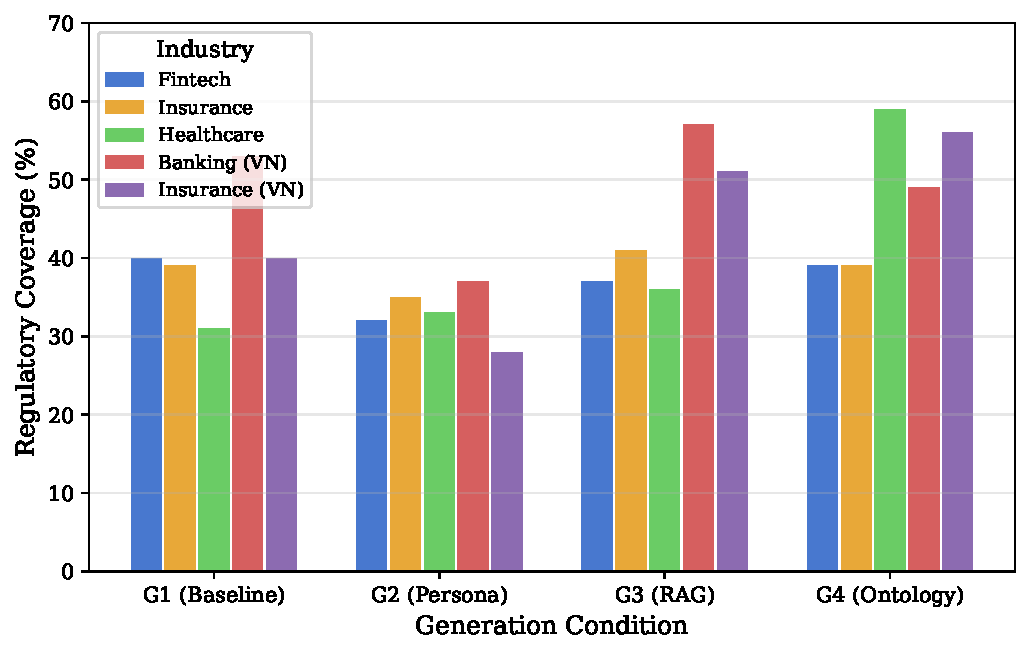
\includegraphics[width=0.85\columnwidth]{figures/rc_by_condition.pdf}
\caption{Regulatory Coverage point estimates by condition and industry. G4 (Ontology) shows the largest point-estimate gains in healthcare (+28pp over G1) and Vietnamese insurance (+16pp); these per-industry G4--G1 differences are not individually Bonferroni-significant but are consistent with the aggregate G4-vs-G2 effect. Banking (VN) favours G3 (RAG), consistent with its denser ontology content.}
\label{fig:rc-by-condition}
\end{figure}

\begin{table}[htbp]
\centering
\caption{Fault Detection Rate by condition (25 faults across 5 industries).
  FDR-design = suite contains a relevant scenario; FDR-execution = fault
  actually detected at runtime. Mean $\pm$ SD across 15 suites per condition.}
\label{tab:fdr-results}
\begin{tabular}{@{}lcccc@{}}
\toprule
\textbf{Metric} & \textbf{G1} & \textbf{G2} & \textbf{G3} & \textbf{G4} \\
\midrule
FDR-design      & .59$\pm$.09 & .57$\pm$.20 & \textbf{.64}$\pm$.22 & .55$\pm$.14 \\
FDR-execution   & .48$\pm$.18 & .53$\pm$.12 & \textbf{.57}$\pm$.10 & .40$\pm$.11 \\
Gap (d $-$ e)   & +.11 & +.04 & +.07 & +.15 \\
\bottomrule
\end{tabular}
\end{table}

\begin{figure}[htbp]
\centering
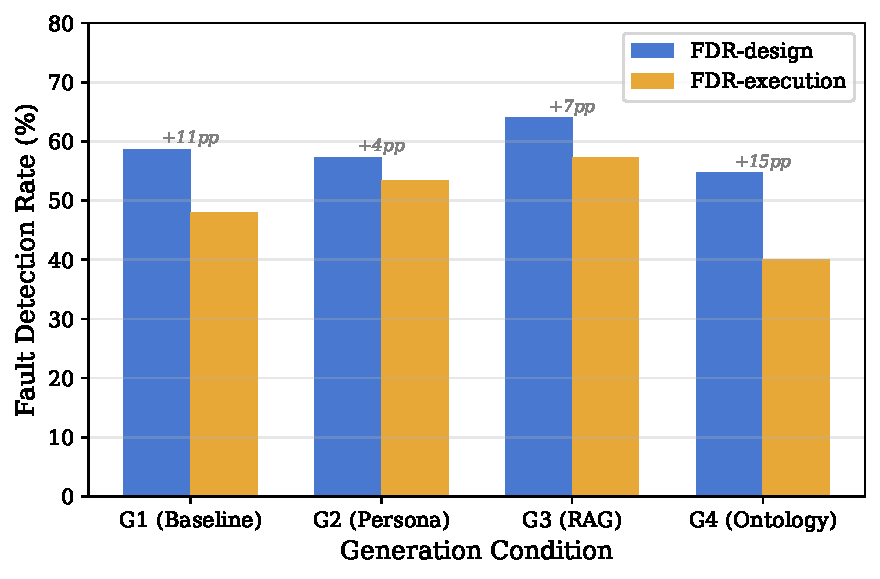
\includegraphics[width=0.75\columnwidth]{figures/fdr_comparison.pdf}
\caption{Fault Detection Rate: design-time coverage vs.\ runtime
  execution. On the Claude pilot, G4 (Ontology) exhibits the largest gap
  (+15pp), suggesting an apparent \emph{coverage-precision tradeoff} on
  this model; \Cref{sec:crossmodel} shows the gap does not replicate on
  Qwen ($-$16pp) or Gemma (+3pp), so the tradeoff is reported as a
  model-dependent observation rather than an established finding.}
\label{fig:fdr-comparison}
\end{figure}

\begin{table}[htbp]
\centering
\caption{Industry Specificity Score (ISS) by condition and industry.
  Mean score on 1--5 Likert scale ($\pm$ SD across 30 scenarios $\times$
  3 replications). Bold = highest per industry.}
\label{tab:iss-results}
\begin{tabular}{@{}lcccc@{}}
\toprule
\textbf{Industry} & \textbf{G1} & \textbf{G2} & \textbf{G3} & \textbf{G4} \\
\midrule
Fintech       & 4.71$\pm$.08 & 4.57$\pm$.03 & 4.77$\pm$.06 & \textbf{4.79}$\pm$.08 \\
Insurance     & 4.34$\pm$.05 & 4.31$\pm$.07 & 4.20$\pm$.03 & \textbf{4.83}$\pm$.03 \\
Healthcare    & 4.54$\pm$.10 & 4.42$\pm$.12 & 4.56$\pm$.20 & \textbf{4.76}$\pm$.07 \\
Banking (VN)  & 4.72$\pm$.17 & 4.73$\pm$.15 & \textbf{4.84}$\pm$.08 & 4.74$\pm$.13 \\
Insurance (VN)& 4.61$\pm$.07 & 4.63$\pm$.03 & 4.73$\pm$.18 & \textbf{4.74}$\pm$.14 \\
\midrule
\textbf{Mean} & 4.59$\pm$.15 & 4.53$\pm$.17 & 4.62$\pm$.25 & \textbf{4.77}$\pm$.04 \\
\bottomrule
\end{tabular}
\end{table}

\begin{figure}[htbp]
\centering
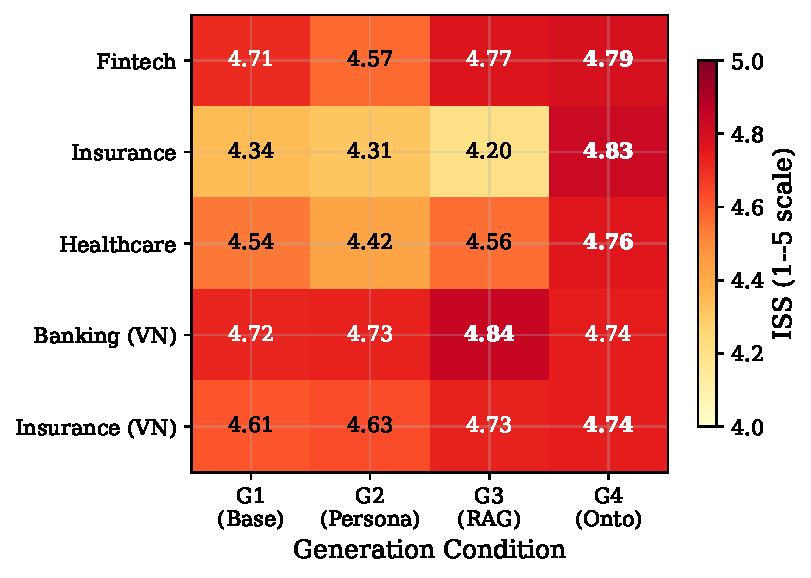
\includegraphics[width=0.7\columnwidth]{figures/iss_heatmap.pdf}
\caption{Industry Specificity Score heatmap by condition and industry.
  Bold values indicate the highest ISS per industry. G4 (Ontology)
  achieves the highest score in 3 of 5 industries; the Insurance
  row shows the largest G4 advantage (+0.63 over G3), demonstrating
  that structured ontology injection produces deeply domain-specific
  scenarios even when RAG-based content yields lower specificity.}
\label{fig:iss-heatmap}
\end{figure}

\begin{table}[htbp]
\centering
\caption{Statistical significance tests (Friedman rank-sum, $k=4$ conditions). Post-hoc: Wilcoxon signed-rank with Bonferroni correction for G4 vs.\ each alternative. Correction is per-DV ($m{=}3$); a family-wise correction over all primary tests would use $m{\approx}12$ (4~DVs~$\times$~3~post-hocs), which leaves G4~$>$~G2 on RC ($p_c{=}.0006$, significant at $\alpha/12$) and G4~$>$~all on ISS ($p_c{<}.001$, significant at $\alpha/12$) but does not change the non-significance of the other G4 comparisons. Kendall's~$W$ effect sizes remain small ($W < 0.07$) across all DVs.}
\label{tab:stats}
\begin{tabular}{@{}lcccl@{}}
\toprule
\textbf{DV} & \textbf{$\chi^2$} & \textbf{$p$-value} &
  \textbf{Kendall's $W$} & \textbf{Verdict (per-DV Bonferroni)} \\
\midrule
RC ($n=125$)  & 15.40 & \textbf{.0015}$^{**}$ & .041 &
  G4 $>$ G2 ($p_c{=}.0006$)$^{***}$; G4 vs.\ G1, G3 n.s. \\
FDR-d ($n=25$) & 0.63 & .891 & .008 & n.s. \\
ISS ($n=150$) & 29.45 & \textbf{$2{\times}10^{-6}$}$^{***}$ & .065 &
  G4 $>$ all ($p_c{<}.001$)$^{***}$ \\
AC ($n=6$)    & 0.07 & .995 & .004 & Equivalent (as predicted) \\
\bottomrule
\end{tabular}
\end{table}

\begin{figure}[htbp]
\centering
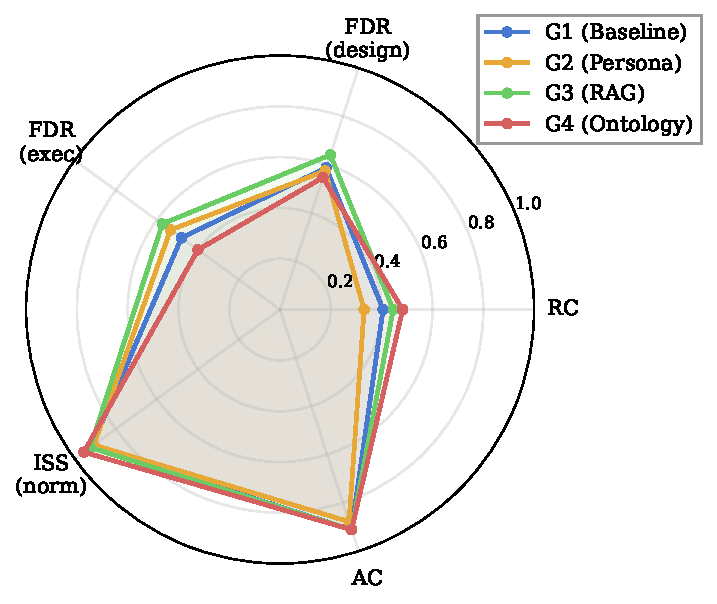
\includegraphics[width=0.55\columnwidth]{figures/summary_radar.pdf}
\caption{Multi-DV summary radar chart (point estimates, normalised). G4 (Ontology) leads on RC (vs.\ G2, Bonferroni-significant) and ISS (vs.\ all, Bonferroni-significant) but shows the lowest FDR-execution in this pilot---an exploratory, model-dependent coverage-precision observation (see Discussion). All conditions achieve near-equivalent AC and FDR-design scores.}
\label{fig:summary-radar}
\end{figure}

\paragraph{Interpretation.}
The results support two of four hypotheses and reveal an unexpected
finding regarding fault detection.

\emph{H1 (RC): Supported against G2.} Ontology-powered generation (G4)
achieves the highest mean regulatory coverage at 48.3\%, significantly
exceeding persona-based generation (G2, 33.1\%; post-hoc $p_c = 0.0006$).
The largest per-industry point-estimate gains over G1 occur in healthcare
(+28pp) and Vietnamese insurance (+16pp), suggesting that ontology value
scales with regulatory complexity; these are descriptive contrasts only,
as the G4 vs.\ G1 omnibus comparison is not Bonferroni-significant
($p_c = 0.243$). The G4 vs.\ G3 difference (+3.7pp) is likewise not
statistically significant after correction ($p_c = 1.0$), indicating that
\emph{structured} ontology and \emph{unstructured} RAG chunks yield similar
coverage when the underlying content is equivalent---a finding we discuss
further in \Cref{sec:discussion}.

\emph{H2 (FDR): Not supported.} Fault detection rates show no
significant differences across conditions ($p = .891$). All conditions
generate scenarios capable of detecting approximately 55--64\% of
injected faults at the design level. However, on the Claude pilot G4
shows the lowest \emph{execution} FDR (40\%) and largest design-execution
gap (+15pp), suggesting that ontology-generated scenarios, while
regulatory-comprehensive, may be less effective at \emph{triggering}
specific fault behaviors at runtime. On Claude this pattern resembles a
\textbf{coverage-precision tradeoff}---breadth (regulatory coverage)
purchased at the expense of depth (fault-triggering precision)---but
\Cref{sec:crossmodel} shows the gap does not replicate on Qwen
($-$16pp) or Gemma (+3pp), so we report the tradeoff as a
model-dependent, exploratory observation rather than an established finding.

\emph{H3 (ISS): Strongly supported.} G4 produces the most
industry-specific scenarios (4.77/5.0), significantly exceeding all
alternatives: G1 ($p_c = 3.2 \times 10^{-5}$), G2 ($p_c < 10^{-5}$),
and G3 ($p_c = 0.0008$). The G4-over-G3 ISS gap is significant
despite comparable RC scores, indicating that structured ontology
injection produces scenarios that are regulatory-relevant
\emph{and} domain-specific in their formulation.

\emph{H4 (AC): Supported.} Adversarial coverage is equivalent across
conditions ($p = .995$, $W = .004$), confirming that adversarial
scenario generation depends on explicit prompting rather than domain
knowledge source. All conditions achieve 88--91\% coverage of the
six-category adversarial taxonomy.

% ----------------------------------------------------------------------------
% 6.2.8 Cross-Model Validation (was 8.8)
% ----------------------------------------------------------------------------
\subsubsection{Cross-Model Validation}
\label{sec:crossmodel}

A key threat to the preceding results is that the ontology advantage
might reflect model-specific parametric knowledge rather than the
structural contribution of ontological context. To address this, we
replicated the full 60-suite experiment with two additional generator
models---Qwen~2.5 72B~Instruct (via OpenRouter) and Gemma~4 26B
(via Google AI Studio)---while holding the Claude Sonnet~4 judge
fixed at $T{=}0.0$ to preserve measurement consistency. The identical
experimental design (4~conditions $\times$ 5~industries $\times$
3~replications $\times$ 30~scenarios) yields 1,800 scenarios per
model and 5,400 total across all three.

\Cref{tab:crossmodel} summarizes the G4 (ontology) performance
across generator models.

\begin{table}[ht]
\centering
\caption{Cross-model comparison of G4 (ontology-powered) generation.
Judge is Claude Sonnet~4 ($T{=}0.0$) for all models.}
\label{tab:crossmodel}
\small
\begin{tabular}{lcccccc}
\toprule
& \multicolumn{2}{c}{\textbf{RC}} & \multicolumn{2}{c}{\textbf{ISS}} & \multicolumn{2}{c}{\textbf{FDR}} \\
\cmidrule(lr){2-3} \cmidrule(lr){4-5} \cmidrule(lr){6-7}
\textbf{Generator} & G4 & $\Delta$(G4$-$G2) & G4 & $\chi^2$ & Design & Exec \\
\midrule
Claude Sonnet~4 & 48.3\% & +15.2pp & 4.77 & 29.4*** & 54.7\% & 40.0\% \\
Gemma~4 26B     & 40.3\% & +11.2pp & 4.68 & 70.1*** & 53.3\% & 50.7\% \\
Qwen~2.5 72B    & 30.1\% & +14.4pp & 4.37 & 103.2*** & 40.0\% & 56.0\% \\
\bottomrule
\multicolumn{7}{l}{\footnotesize ***\,$p < .001$ (Friedman omnibus for ISS H3)}
\end{tabular}
\end{table}

\paragraph{H5 (RC advantage replicates).}
All three models show G4 significantly exceeding G2 on regulatory
coverage: Claude ($\Delta{=}+15.2$pp, $p_c{=}.0006$), Gemma
($\Delta{=}+11.2$pp, $p_c{=}.009$), and Qwen
($\Delta{=}+14.4$pp, $p_c{=}.005$). The ontology advantage is
\emph{universal}---not an artifact of Claude's parametric knowledge.

\paragraph{H6 (ISS advantage replicates).}
G4 achieves the highest industry specificity score across all three
models: Claude (4.77/5.0), Gemma (4.68/5.0), and Qwen (4.37/5.0),
each with omnibus $p < 10^{-5}$. For Qwen, all three post-hoc
comparisons (G4 vs.\ G1, G2, G3) are significant at Bonferroni-corrected
$p < .001$. The ISS gap between models is smallest for G4 (range:
0.40 across models) versus G1 (range: 0.42), suggesting that
\emph{ontology partially compensates for model capability differences}.

\paragraph{H7 (Coverage-precision tradeoff).}
The FDR design-execution gap varies by model: Claude shows a positive
gap (+14.7pp: design overestimates execution), Gemma shows a near-zero
gap (+2.7pp), and Qwen shows a negative gap ($-$16.0pp: execution
outperforms design). This reveals that the coverage-precision tradeoff
identified in the Claude-only analysis (\Cref{sec:empirical}) is
\emph{not universal} but rather a model-dependent interaction between
ontological structure and the generator's ability to translate
regulatory-coverage scenarios into fault-triggering test cases.

\paragraph{Exploratory three-model observation.}
Absolute G4 RC orders Claude $>$ Gemma $>$ Qwen (48.3\% $>$ 40.3\% $>$ 30.1\%), and ISS similarly (4.77 $>$ 4.68 $>$ 4.37). The G4-minus-G1 RC uplift, however, shows a different ordering: Qwen (+12.0pp) $>$ Claude (+7.7pp) $>$ Gemma (+3.7pp). H8 from our cross-model protocol---``lower-capability models benefit disproportionately from ontological context''---is thus \emph{directionally consistent} with the Inverse Parametric Knowledge Effect reported in our companion study \citep{luong2026neurosymbolic}, but we flag three caveats: (i)~$n{=}3$ model points cannot establish a general model-family-level claim; (ii)~the capability-proxy ordering (Gemma 26B vs Qwen 72B) is non-monotone in parameter count, so ``baseline capability'' must be read as in-study G1~RC rather than model scale; (iii)~using in-study G1~RC as the capability axis makes H8 partially tautological (low-G1 models have more headroom). We therefore present the three-model gradient as an \emph{exploratory observation} that motivates the $\geq$6-model replication proposed in future work, not as a confirmed finding.

\begin{figure}[htbp]
\centering
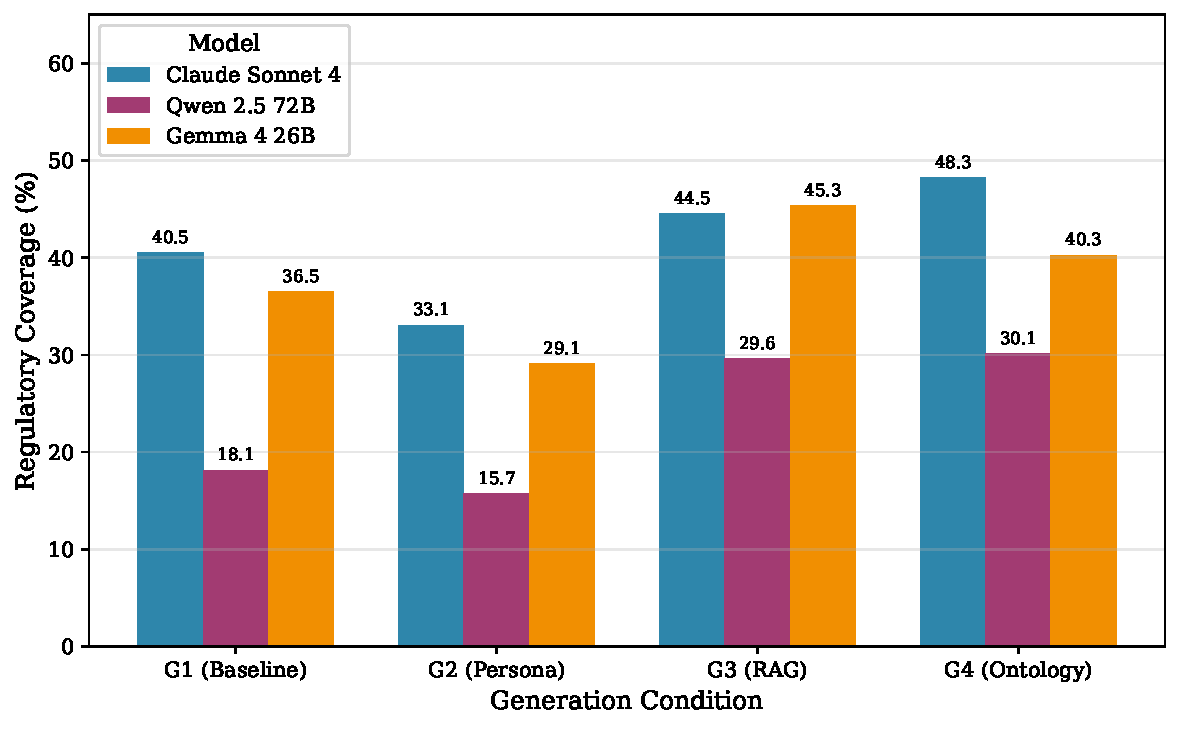
\includegraphics[width=\columnwidth]{figures/crossmodel_rc.pdf}
\caption{Regulatory Coverage (RC) by generation condition across three
  generator models. G4 (ontology) achieves the highest RC for all
  models, confirming that the ontology advantage is not
  model-specific.}
\label{fig:crossmodel-rc}
\end{figure}

\begin{figure}[htbp]
\centering
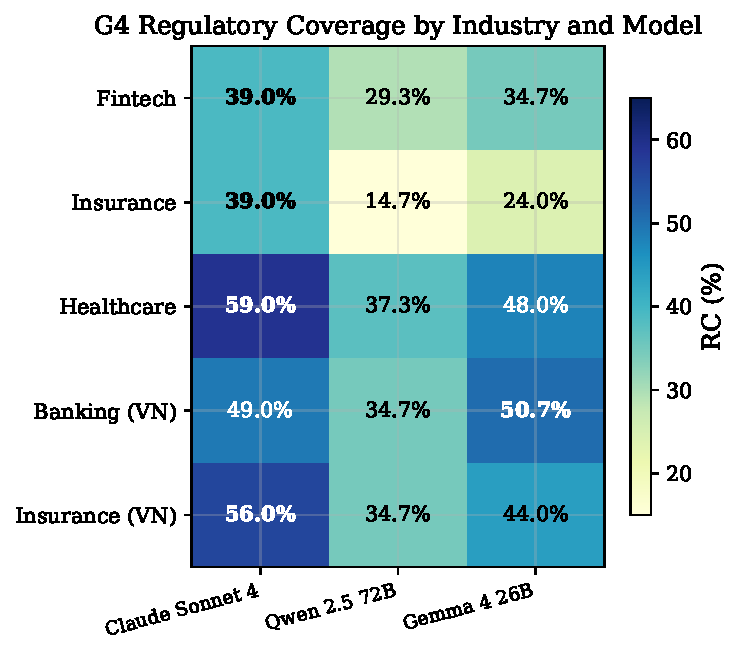
\includegraphics[width=\columnwidth]{figures/crossmodel_rc_heatmap.pdf}
\caption{G4 Regulatory Coverage by industry and generator model.
  Claude achieves the highest absolute RC across most industries,
  while the ontology uplift is largest for models with lower baseline
  capability (Qwen), consistent with the Inverse Parametric Knowledge
  Effect.}
\label{fig:crossmodel-rc-heatmap}
\end{figure}

% ============================================================================
% 7. DISCUSSION (was Section 10; Section 9 Continuous Optimization removed
% per chair review of v0.8)
% ============================================================================
\section{Discussion}
\label{sec:discussion}

\subsection{Ontology as Specification Language}

A key insight of this work is that enterprise ontologies serve a
\emph{triple} purpose in the agent lifecycle:

\begin{enumerate}
  \item \textbf{Grounding} (\emph{input}): The ontology provides
    structured context that improves agent reasoning---validated
    empirically in our RA-3 companion study
    \citep{luong2026neurosymbolic}.

  \item \textbf{Specification} (\emph{test generation}): The same
    ontology generates the test scenarios that verify agent
    behavior---the scenario generation algorithm of
    \Cref{sec:scenario-generation}, validated in
    \Cref{sec:empirical}.

  \item \textbf{Oracle} (\emph{evaluation}): The ontology provides
    the evaluation criteria against which the LLM judge assesses
    agent responses---the regulatory checklists and domain-specific
    rubrics.
\end{enumerate}

\noindent This triple role connects to the model-based testing
paradigm \citep{utting2012taxonomy}: in MBT, the model serves as
both specification and oracle. We extend this by adding the
grounding role---the ontology not only defines what to test and how
to evaluate, but also \emph{improves the system under test}. This
creates a virtuous cycle: a better ontology produces better agents
\emph{and} more rigorous verification, with measurable coverage
guarantees that traditional prompt engineering cannot provide.

\subsection{The LLM-as-Judge Limitation}

Our current evaluation approach uses an LLM as the judge for
scenario assessment. This introduces a meta-level concern: can
we trust an LLM to accurately evaluate another LLM's compliance
with regulatory requirements? We mitigate this through:

\begin{enumerate}
  \item \textbf{Structured evaluation criteria}: The judge receives
    explicit, per-regulation evaluation rubrics derived from the
    ontology, reducing the scope for subjective interpretation.
  \item \textbf{Deterministic checks where possible}: Numeric
    threshold compliance (e.g., ``is the amount above \$10,000?'')
    is checked programmatically, not by the LLM judge.
  \item \textbf{Human review of failures}: All failed scenarios
    are flagged for human review so that false negatives surface.
\end{enumerate}

Long-term, we envision replacing LLM-as-judge with formal
verification methods (V4--V5 in our spectrum) for the most
critical properties.

\subsection{Comparison with Lyzr A-SIM}

Our ontology-powered approach offers several advantages over
Lyzr's persona-scenario matrix approach:

\begin{table}[htbp]
\centering
\caption{Comparison: Ontology-Powered vs. Persona-Scenario
  Simulation.\textsuperscript{$\dagger$}}
\label{tab:comparison}
\begin{tabular}{@{}lcc@{}}
\toprule
\textbf{Dimension} & \textbf{Persona-Scenario} & \textbf{Ontology-Powered} \\
\midrule
Scenario source & Manual + generic & Auto-generated from ontology \\
Industry specificity & Low & High (22 verticals) \\
Regulatory coverage & Incidental & Systematic \\
Coverage metric & Scenario count & Regulatory coverage \% \\
Maintenance & Manual updates & Ontology-driven updates \\
Formal properties & None & LTL-based specification \\
Certification & Pass/fail & Graduated (App/Cond/Rej) \\
\bottomrule
\end{tabular}

\smallskip
\noindent\textsuperscript{$\dagger$}\footnotesize{Ontology-Powered
column reflects the proposed architecture; current \faos{}
implementation uses template-based scenario generation with manual
curation, with full algorithmic generation per
\Cref{alg:scenario-gen} planned.}
\end{table}

\noindent The distinction between persona-scenario and ontology-powered
generation is not architectural but one of \emph{unit of analysis}.
Persona-scenario matrices optimize for \emph{behavioural coverage}:
do the test cases exercise diverse interaction patterns?
Ontology-powered generation optimizes for \emph{regulatory coverage}:
do the test cases verify compliance with the actual regulatory
corpus? Our pilot study (\Cref{sec:empirical})
tests this distinction empirically by measuring both behavioral
dimensions (ISS, AC) and regulatory dimensions (RC, FDR) across
both approaches (G2 = persona-scenario, G4 = ontology-powered).
Our empirical results confirm this prediction: G2 achieves comparable
AC (88\% vs.\ G4's 91\%, $p{=}.995$) but significantly lower RC
(33.1\% vs.\ G4's 48.3\%, post-hoc $p_c{=}.0006$). Persona-scenario
matrices generate behaviorally diverse but regulatory-shallow test
suites.

\subsection{Governance Framework Alignment}

The rapid maturation of AI agent governance in 2025--2026 provides
external validation for our framework's design choices.
The OWASP Top~10 for Agentic Applications \citep{owasp2025agentic}
identifies goal hijacking (ASI01), tool misuse (ASI02), and rogue
agents (ASI10) as critical risks---all of which map directly to
scenario categories in our ontology-to-scenario taxonomy
(\Cref{sec:scenario-generation}): regulatory scenarios test for
goal deviation, operational scenarios exercise tool boundaries, and
adversarial scenarios simulate rogue behavior.

NIST's AI Agent Standards Initiative \citep{nist2026agents} calls
for identity, security, and monitoring standards for autonomous
agents. Our Trust Certificate (\Cref{sec:safety-certificate})
provides a concrete implementation of the ``monitoring and logging''
pillar, while the operational envelope
(\Cref{sec:operational-envelope}) formalizes the ``security and risk
management'' dimension.

The Microsoft Agent Governance Toolkit \citep{microsoft2026agt}
addresses runtime enforcement---policy interception \emph{during}
agent execution. Our framework complements this by addressing
\emph{pre-deployment} verification: ontology-powered simulation
determines \emph{whether} to deploy, while runtime governance
determines \emph{how} to constrain. Together, they form a
defense-in-depth strategy for enterprise AI agent safety.

\subsection{Compositional Verification}
\label{sec:compositional}

Enterprise deployments rarely involve single agents. The \faos{}
platform supports agent teams via the A2A (Agent-to-Agent) protocol
and multi-agent workflow orchestration via LangGraph. This raises the
\emph{compositional verification problem}: given individually
certified agents $\agent_1, \ldots, \agent_n$, what can we conclude
about the safety of their composition?

Classical assume-guarantee reasoning \citep{clarke2018handbook}
provides a foundation: if agent $\agent_i$ is verified under
assumption $A_i$ about its environment (including other agents),
and the composition satisfies all assumptions, then the system-level
properties hold. Formally:

\begin{equation}
  \frac{\forall i: \langle A_i \rangle \agent_i \langle \Phi_i \rangle
    \qquad \bigwedge_i \Phi_i \implies \bigwedge_j A_j}{
    \langle \top \rangle \agent_1 \| \cdots \| \agent_n
    \langle \bigwedge_i \Phi_i \rangle}
\end{equation}

However, LLM-based agents violate a key assumption of classical
compositional verification: their behavior is \emph{not deterministic
given inputs}. The same agent receiving identical messages from
collaborators may produce different outputs across runs. We identify
three research directions to address this:

\begin{enumerate}
  \item \textbf{Probabilistic assume-guarantee}: Extend the
    framework with probabilistic guarantees
    ($P[\Phi_i] \geq 1 - \delta_i$), deriving system-level
    confidence from component-level confidence via independence
    or correlation bounds.

  \item \textbf{Envelope intersection}: Define the composite
    envelope $\env_{\agent_1 \| \cdots \| \agent_n}$ as the
    intersection of individual envelopes, so no agent can drive
    the system outside any co-agent's certified bounds.

  \item \textbf{Protocol-level verification}: Verify the
    \emph{interaction protocol} (message types, sequencing,
    escalation rules) independently of agent internals, using
    the A2A protocol specification as a checkable contract.
\end{enumerate}

Compositional verification is not addressed in the current \faos{}
implementation and constitutes a significant direction for future work.

% ============================================================================
% 8. LIMITATIONS (promoted from former Section 10.5 per chair review;
% Section 11 Threats to Validity removed per chair review)
% ============================================================================
\section{Limitations}
\label{sec:limitations}

Three limitations bound the conclusions of this work.
\emph{First, ontology completeness:} verification coverage is bounded
by ontology coverage---a regulation absent from the ontology creates
a systematic blind spot, placing a continuing curation burden on
enterprise adopters as a precondition for trust.
\emph{Second, LLM-as-judge construct validity:} the evaluation
pipeline uses Claude Sonnet~4 as both generator and fixed judge
($T{=}0.0$), introducing potential self-enhancement bias that
cross-generator replication alone cannot eliminate (see
\Cref{sec:crossmodel}); a related concern is that the same author
designed both the FAOS ontology and the regulatory checklist used as
ground truth, making the anti-circularity control (E1) a pseudo-control
rather than a fully independent check. Deterministic evaluation,
ontology-derived binary rubrics, programmatic threshold checks (e.g.\
the \$10{,}000 CTR line), and three-model cross-validation partially
mitigate these risks, but inter-judge and inter-rater triangulation
remain the dominant residual concerns.
\emph{Third, statistical confidence versus formal guarantees:}
simulation establishes practical assurance at verification levels
V1--V3, but higher levels (V4--V5) may be computationally intractable
for agents with large state spaces (\Cref{sec:formal-extensions}).
The graduated verdict thresholds
($\theta_{\text{high}}{=}0.95$, $\theta_{\text{low}}{=}0.80$) also
remain illustrative engineering parameters, not yet calibrated
against real-world deployment incident rates, and no agent in the
pilot corpus satisfied $\theta_{\text{high}}$.

These limitations chart a concrete future-work agenda. Inter-rater
validation of the 125-item regulatory checklist by non-author
regulatory experts on a stratified random sample, paired with
non-Anthropic judge triangulation (GPT-4o or Gemini) on the same
sub-sample and reported judge--judge agreement metrics for each
dependent variable, will quantify residual self-enhancement bias and
re-anchor effect-size estimates accordingly. Scaling cross-model
replication to six or more LLM families under an independent
capability proxy (MMLU score or training-token count) will test
whether the cross-model coverage-precision pattern is intrinsic to the
ontology approach or an artefact of the present three-model sample;
the disaggregated seen-vs-unseen regulatory-coverage split, released
with the v0.2 artifact at paper acceptance, supports this scaling
exercise. Executing runtime verification (V3) and probabilistic
bounded model checking (V2) on production-deployed agents will move
the framework from \emph{proposed} to \emph{delivered} attestation,
while extending to multi-agent settings via probabilistic
assume-guarantee contracts over the A2A protocol will broaden the
certification surface to agent teams. Calibrating the verdict
thresholds against actual deployment incident rates and publishing a
Trust Certificate registry that links specific agent versions to
their verification evidence will close the gap between the proposed
framework and an operational deployment gate. Together, these
directions advance the state of practice from reactive runtime
control toward systematic pre-deployment assurance for enterprise
Agentic AI.

% ============================================================================
% 9. CONCLUSION (was Section 12)
% ============================================================================
\section{Conclusion and Future Work}
\label{sec:conclusion}

This study proposes a pre-deployment verification framework for
enterprise AI agents that combines ontology-grounded scenario
generation, operational-envelope specification, and a proposed Trust
Certification model for deployment assurance in regulated
environments. The framework introduces three connected contributions:
(i)~the \emph{Agent Operational Envelope}, which formalises the scope
within which an agent is evaluated and authorised to operate; (ii)~an
\emph{ontology-to-scenario generation pipeline} that systematically
derives regulatory, operational, and adversarial test cases; and
(iii)~a \emph{machine-verifiable Trust Certification architecture}
with graduated deployment verdicts and a five-level verification
spectrum extending toward formal methods.

The empirical results demonstrate that ontology-grounded generation
substantially improves regulatory coverage and domain specificity
relative to persona-based simulation approaches. In a controlled pilot
spanning four regulated industries (Fintech, Banking, Insurance,
Healthcare) instantiated as five industry-by-regulatory-regime cells,
1{,}800 scenarios, 125 primary-source regulatory requirements, and
25 injected faults, the ontology-powered approach (G4) achieved
48.3\% regulatory coverage versus 33.1\% for the dominant
persona-scenario baseline (G2; $p_c{=}.0006$) and the highest
industry specificity (4.77/5.0; $p{=}2{\times}10^{-6}$), while the
regulatory-coverage advantage over the plain-prompt baseline (G1)
and RAG-augmented prompting (G3) is not Bonferroni-robust. Cross-validation across three distinct LLM
families (Claude Sonnet~4, Qwen~2.5 72B, and Gemma~4 26B; 5{,}400
total scenarios) replicated the core persona-versus-ontology pattern,
alongside an exploratory, model-dependent coverage-precision
observation on fault detection, suggesting that the observed gains
arise from structural properties of the verification methodology
rather than from a single model family.

At the same time, the study deliberately distinguishes statistical
assurance from formal guarantees. The proposed Trust Certification
framework remains conceptual at higher verification levels, ontology
completeness constrains verification coverage, and the fixed
LLM-as-judge design leaves residual self-enhancement bias unresolved.
These limitations define the next phase of research: independent
evaluator triangulation, broader cross-model replication under an
independent capability proxy, probabilistic verification for
multi-agent systems via assume-guarantee contracts over the A2A
protocol, and progression from simulation-based evidence toward
formally grounded deployment assurance.

More broadly, the results suggest that enterprise AI governance may
require a transition from reactive runtime control toward systematic
pre-deployment verification. Current enterprise practice largely
assumes that monitoring, guardrails, and human oversight can
compensate for insufficient pre-deployment assurance. This work argues
instead for a verification-first paradigm in which autonomous agents
are evaluated against explicit operational, regulatory, and safety
constraints before deployment. In this context, ontology-grounded
simulation represents a practical and scalable step toward
enterprise-grade trust infrastructure for Agentic AI systems.

% ============================================================================
% ACKNOWLEDGMENTS
% ============================================================================
\section*{Acknowledgments}

The authors thank the FAOS team for platform access and ontology
content used in the empirical evaluation.

% ============================================================================
% DATA AVAILABILITY
% ============================================================================
\paragraph{Data availability.}
The dataset comprises 5,400 generated scenarios across three
generator models (Claude Sonnet~4, Qwen~2.5 72B, Gemma~4 26B),
each contributing 1,800 scenarios from 60 test suites
(4~conditions $\times$ 5~industries $\times$ 3~replications $\times$
30~scenarios). Per-model assessments include 125 regulatory coverage
evaluations per condition, 25 fault injection results, and 150
industry specificity scores per condition---all judged by a fixed
Claude Sonnet~4 evaluator ($T{=}0.0$). Analysis scripts, ontology
context files, regulatory checklists, fault definitions, and
cross-model analysis code are publicly available at the FAOS Research
repository \citep{faos-research-repo}. Raw scenario data and judge
evaluation logs will be released with the v0.2 artifact at paper acceptance.

% ============================================================================
% REFERENCES
% ============================================================================
\bibliography{references}

\end{document}
